本研究で構築した現在のアプリは、マイクロサービス的な疎結合アーキテクチャを採用し、スケーラビリティと保守性を重視した設計となっている。図\ref{fig:architecture}に全体構成を示す。

\begin{figure}[htbp]
\centering
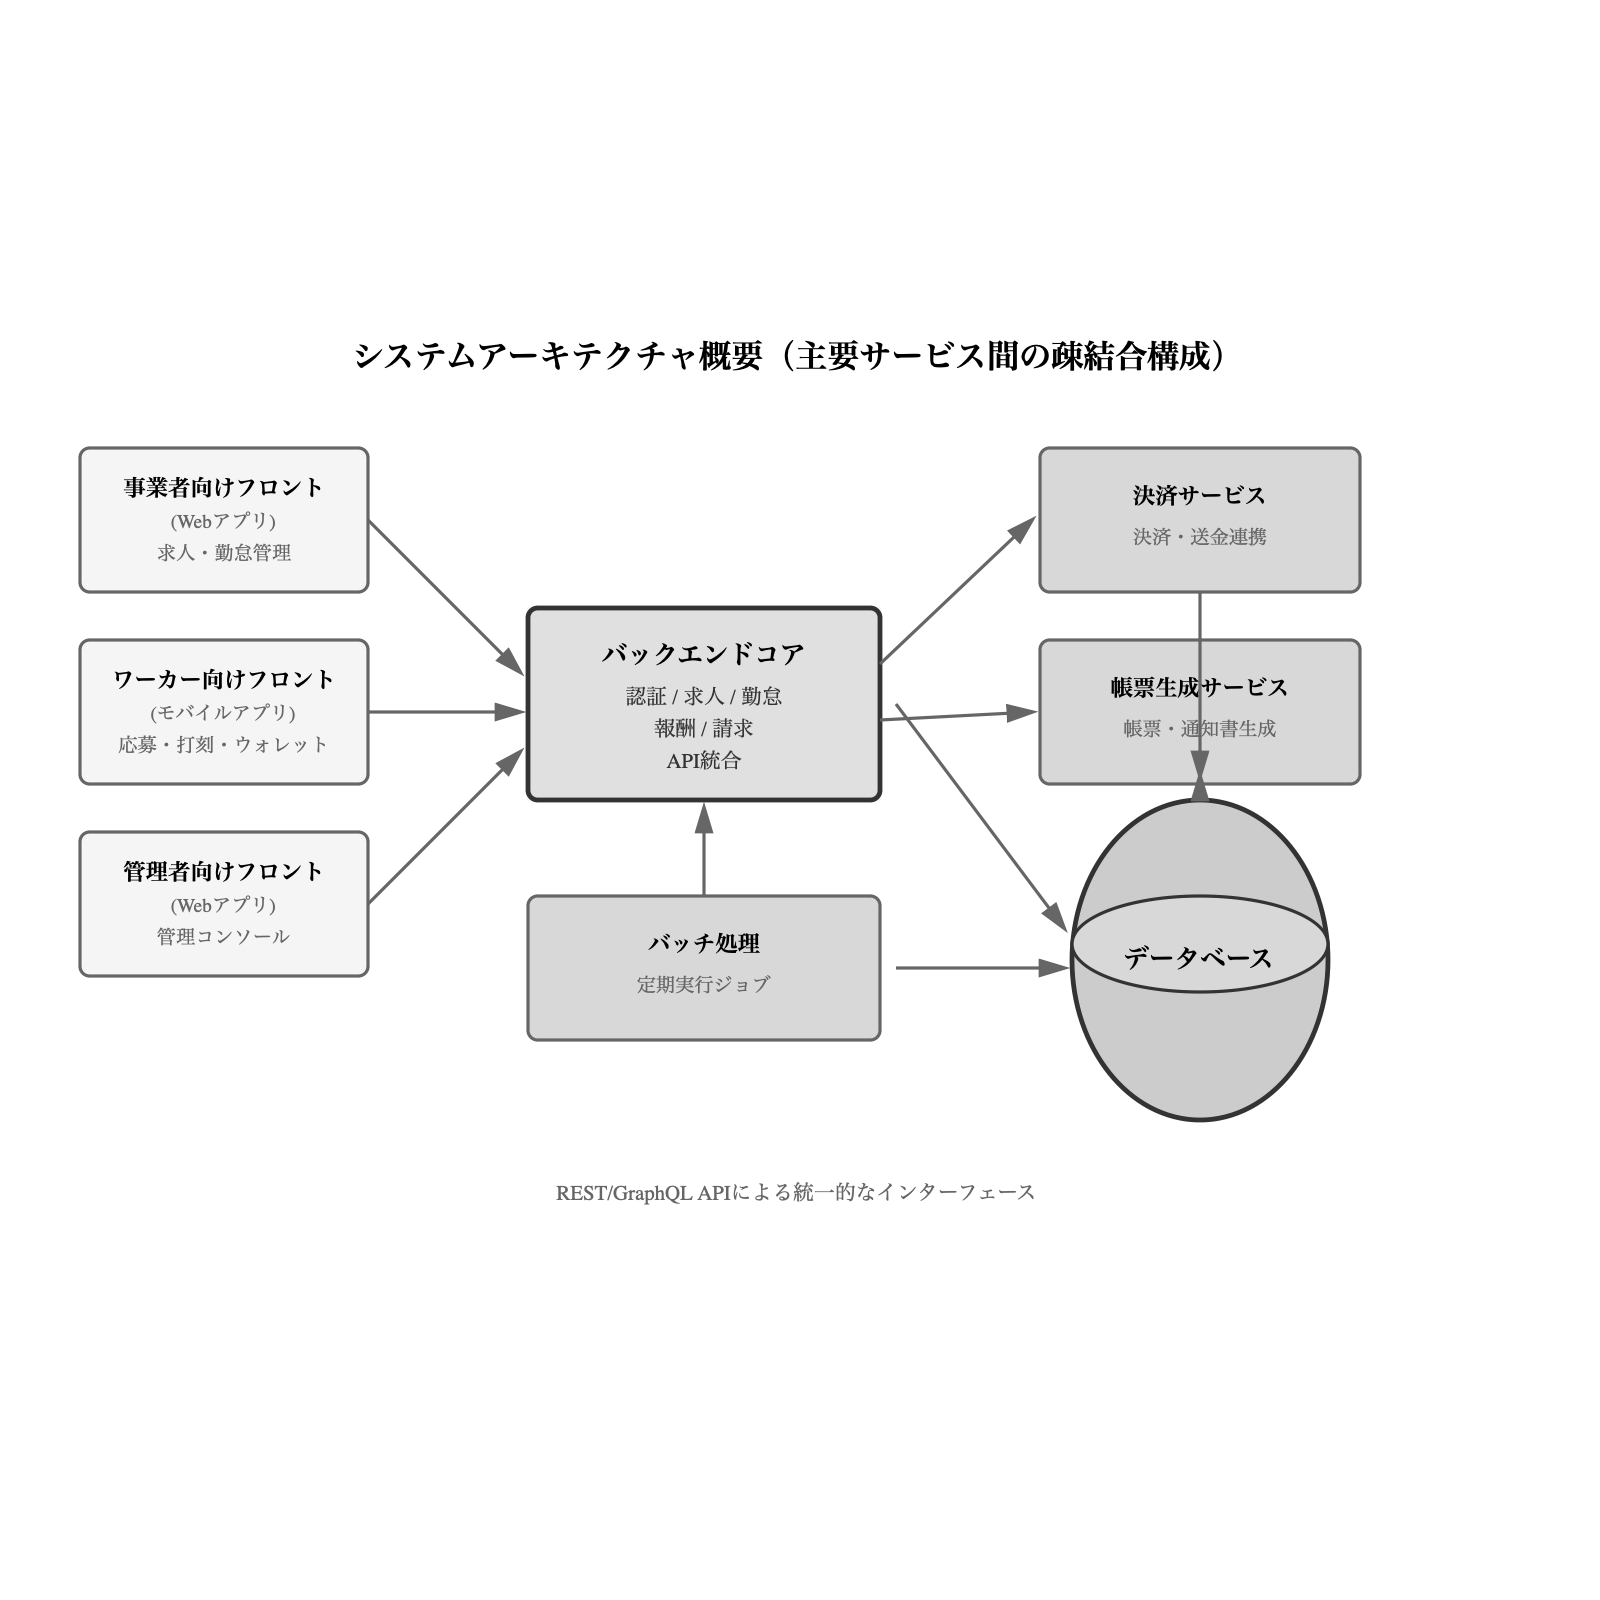
\includegraphics[width=0.95\textwidth]{images/fig_architecture.png}
\caption{システムアーキテクチャ概要（主要サービス間の疎結合構成）}
\label{fig:architecture}
\end{figure}

設計の主要な特徴として、（1）\textbf{関心事の分離}：事業者向け・ワーカー向け・管理者向けの各フロントエンドを独立開発可能とし、異なる技術スタック（Angular/Flutter）を採用できる柔軟性を確保した。（2）\textbf{決済処理の分離}：金銭を扱う決済サービスを独立させることで、セキュリティ要件やPCI DSS準拠を局所化し、他サービスへの影響を最小化した。（3）\textbf{バッチ処理の独立性}：日次・月次の定期処理をcron-jobsとして分離し、リアルタイムAPIサーバーへの負荷を回避した。（4）\textbf{統一的なデータベース}：複数サービス間でデータベースを共有することで、データの一貫性を保ちつつ、各サービスは必要なコレクションのみにアクセスする。この構成により、マッチングアルゴリズムの改善やNLPモデルの追加といった機能拡張を、既存サービスへの影響を最小限に抑えながら実施できる。
